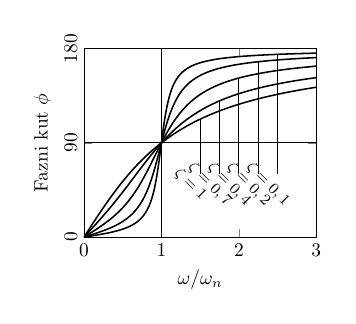
\begin{tikzpicture}[scale=0.7]
	\begin{axis} [
		height=5cm,
		ylabel = Fazni kut $\phi$, 
		xlabel = $\omega/\omega_n$,
		xmin = 0,
		xmax = 3,
		ymin = 0,
		ymax = 180,
		xtick = {0,1,2,3}, 
		ytick = {0,90,180}, yticklabel style={rotate=90},
	]

            \foreach \i in {1, 0.7, 0.4, 0.2, 0.1}
            {
                \addplot [
                    domain=0:1,
                    samples=200,
                    color=black,
                    thick
                ]{atan((2*x*\i)/(1-x^2))};
            }

            \foreach \i in {1, 0.7, 0.4, 0.2, 0.1}
            {
                \addplot [
                    domain=1.001:3,
                    samples=200,
                    color=black,
                    thick
                ]{180+atan((2*x*\i)/(1-x^2))};
            }
            \draw[thin](1.5,{180+atan((2*1.5*1)/(1-1.5^2))}) -- (1.5, 60)
                node[pos=1,rotate=-45,below] {\footnotesize{$\zeta=1$}};
            \draw[thin](1.75,{180+atan((2*1.75*0.7)/(1-1.75^2))}) -- (1.75, 60)
                node[pos=1,rotate=-45,below] {\footnotesize{$\zeta=0,7$}};
            \draw[thin](2,{180+atan((2*2*0.4)/(1-2^2))}) -- (2, 60)
                node[pos=1,rotate=-45,below] {\footnotesize{$\zeta=0,4$}};
            \draw[thin](2.25,{180+atan((2*2.25*0.2)/(1-2.25^2))}) -- (2.25, 60)
                node[pos=1,rotate=-45,below] {\footnotesize{$\zeta=0,2$}};
            \draw[thin](2.5,{180+atan((2*2.5*0.1)/(1-2.5^2))}) -- (2.5, 60)
                node[pos=1,rotate=-45,below] {\footnotesize{$\zeta=0,1$}};



        \draw[thin](1,0)--(1,180);
        \draw[thin](0,90) -- (3,90);
        \end{axis}
\end{tikzpicture}
